\section{Approximate Inductance Formula}

The model is
\[
\hat L=\alpha n^{\beta_1}w^{\beta_2}d^{\beta_3}D^{\beta_4}
\]
Taking logs gives a linear least-squares problem:
\[
\log \hat L_i
=
\log\alpha+\beta_1\log n_i+\beta_2\log w_i+\beta_3\log d_i+\beta_4\log D_i
\]
Define
\[
\theta=
\begin{bmatrix}
\log\alpha\\ \beta_1\\ \beta_2\\ \beta_3\\ \beta_4
\end{bmatrix},
\qquad
X_i=
\begin{bmatrix}
1&\log n_i&\log w_i&\log d_i&\log D_i
\end{bmatrix}
\]
and \(z_i=\log L_i\). The model can be fitted by minimizing
\[
\|X\theta-z\|_2^2
\]
This minimizes the sum of squared log-errors, which is a natural criterion here because the model is multiplicative and the final error is relative to the true inductance.

% The fitted parameters are
% \[
% \alpha=7.0725326\times 10^{-4}
% \]
% \[
% \beta_1=1.3793645,\qquad
% \beta_2=-0.48060387,\qquad
% \beta_3=0.27561595,\qquad
% \beta_4=1.2131716
% \]
% Thus
% \[
% \hat L
% =
% 7.0725326\times 10^{-4}
% n^{1.3793645}
% w^{-0.48060387}
% d^{0.27561595}
% D^{1.2131716}
% \]

% The average percentage error is
% \[
% \frac{1}{50}\sum_{i=1}^{50}100\frac{|\hat L_i-L_i|}{L_i}
% =6.7700\%
% \]
% The maximum percentage error over the 50 inductors is
% \[
% 19.2509\%
% \]

\begin{figure}[H]
    \centering
    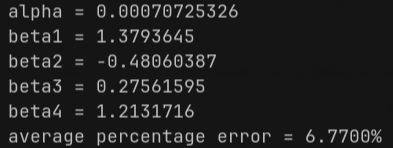
\includegraphics[width=0.6\textwidth]{img/p5.png}
\end{figure}

% \begin{figure}[H]
%     \centering
%     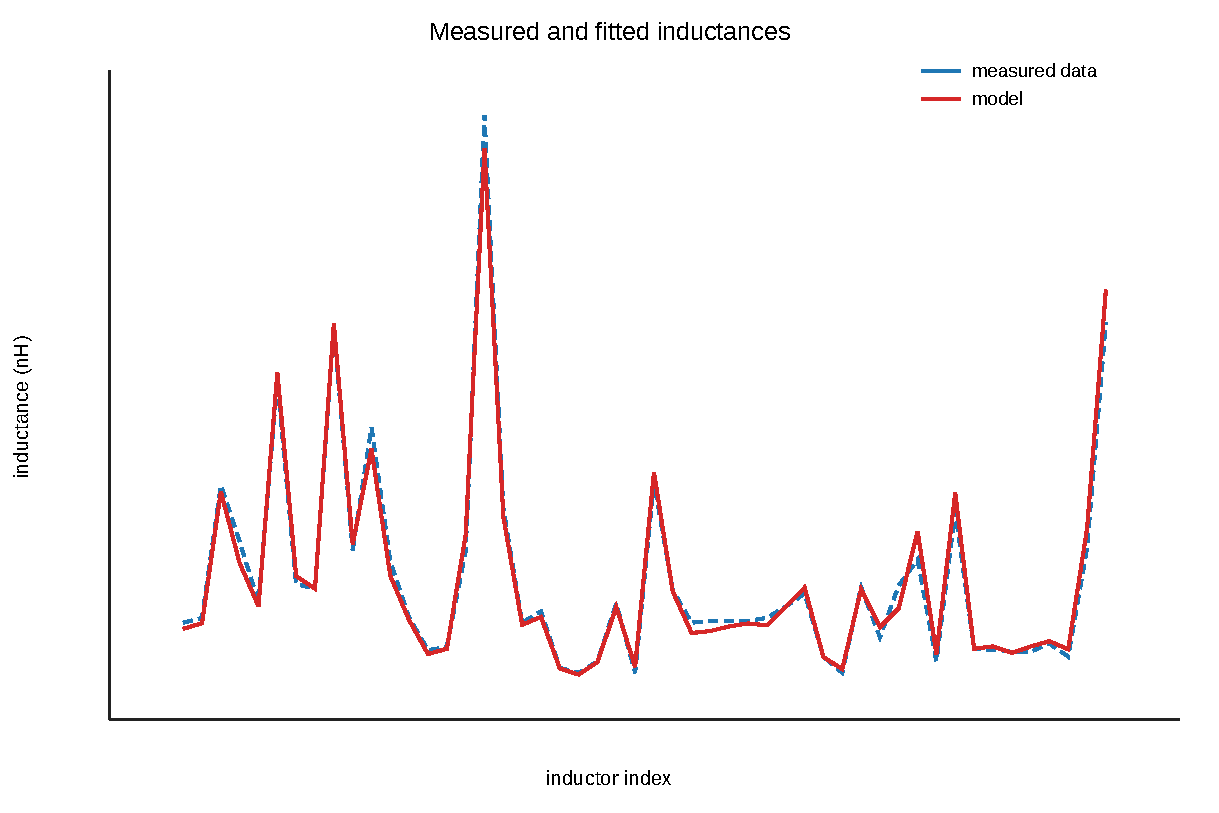
\includegraphics[width=0.82\textwidth]{img/p5_inductor_fit.pdf}
%     \caption{Measured inductances and fitted multiplicative model}
% \end{figure}

\subsection{Code}
\begin{lstlisting}[language={}]
using LinearAlgebra
using Statistics

include(joinpath(@__DIR__, "readclassjson.jl"))

data = readclassjson(joinpath(@__DIR__, "inductor_data.json"))
nturns = data["n"]
w = data["w"]
d = data["d"]
D = data["D"]
L = data["L"]

X = hcat(ones(length(L)), log.(nturns), log.(w), log.(d), log.(D))
theta = X \ log.(L)

alpha = exp(theta[1])
beta = theta[2:end]

Lhat = exp.(X * theta)
pct_error = 100 .* abs.(Lhat .- L) ./ L

average_error = mean(pct_error)
\end{lstlisting}
